%Version 3.1 December 2024
% See section 11 of the User Manual for version history
%
%%%%%%%%%%%%%%%%%%%%%%%%%%%%%%%%%%%%%%%%%%%%%%%%%%%%%%%%%%%%%%%%%%%%%%
%%                                                                 %%
%% Please do not use \input{...} to include other tex files.       %%
%% Submit your LaTeX manuscript as one .tex document.              %%
%%                                                                 %%
%% All additional figures and files should be attached             %%
%% separately and not embedded in the \TeX\ document itself.       %%
%%                                                                 %%
%%%%%%%%%%%%%%%%%%%%%%%%%%%%%%%%%%%%%%%%%%%%%%%%%%%%%%%%%%%%%%%%%%%%%

%%\documentclass[referee,sn-basic]{sn-jnl}% referee option is meant for double line spacing

%%=======================================================%%
%% to print line numbers in the margin use lineno option %%
%%=======================================================%%

%%\documentclass[lineno,pdflatex,sn-basic]{sn-jnl}% Basic Springer Nature Reference Style/Chemistry Reference Style

%%=========================================================================================%%
%% the documentclass is set to pdflatex as default. You can delete it if not appropriate.  %%
%%=========================================================================================%%

%%\documentclass[sn-basic]{sn-jnl}% Basic Springer Nature Reference Style/Chemistry Reference Style

%%Note: the following reference styles support Namedate and Numbered referencing. By default the style follows the most common style. To switch between the options you can add or remove “Numbered” in the optional parenthesis. 
%%The option is available for: sn-basic.bst, sn-chicago.bst%  
 
%%\documentclass[pdflatex,sn-nature]{sn-jnl}% Style for submissions to Nature Portfolio journals
%%\documentclass[pdflatex,sn-basic]{sn-jnl}% Basic Springer Nature Reference Style/Chemistry Reference Style
\documentclass[pdflatex,sn-mathphys-num]{sn-jnl}% Math and Physical Sciences Numbered Reference Style
%%\documentclass[pdflatex,sn-mathphys-ay]{sn-jnl}% Math and Physical Sciences Author Year Reference Style
%%\documentclass[pdflatex,sn-aps]{sn-jnl}% American Physical Society (APS) Reference Style
%%\documentclass[pdflatex,sn-vancouver-num]{sn-jnl}% Vancouver Numbered Reference Style
%%\documentclass[pdflatex,sn-vancouver-ay]{sn-jnl}% Vancouver Author Year Reference Style
%%\documentclass[pdflatex,sn-apa]{sn-jnl}% APA Reference Style
%%\documentclass[pdflatex,sn-chicago]{sn-jnl}% Chicago-based Humanities Reference Style

%%%% Standard Packages
%%<additional latex packages if required can be included here>

\usepackage[utf8]{inputenc}
\usepackage{graphicx}%
\usepackage{multirow}%
\usepackage{amsmath,amssymb,amsfonts}%
\usepackage{amsthm}%
\usepackage{mathrsfs}%
\usepackage[title]{appendix}%
\usepackage{xcolor}%
\usepackage{textcomp}%
\usepackage{manyfoot}%
\usepackage{booktabs}%
\usepackage{algorithm}%
\usepackage{algorithmicx}%
\usepackage{algpseudocode}%
\usepackage{listings}%
\usepackage{subcaption}
%%%%

%%%%%=============================================================================%%%%
%%%%  Remarks: This template is provided to aid authors with the preparation
%%%%  of original research articles intended for submission to journals published 
%%%%  by Springer Nature. The guidance has been prepared in partnership with 
%%%%  production teams to conform to Springer Nature technical requirements. 
%%%%  Editorial and presentation requirements differ among journal portfolios and 
%%%%  research disciplines. You may find sections in this template are irrelevant 
%%%%  to your work and are empowered to omit any such section if allowed by the 
%%%%  journal you intend to submit to. The submission guidelines and policies 
%%%%  of the journal take precedence. A detailed User Manual is available in the 
%%%%  template package for technical guidance.
%%%%%=============================================================================%%%%

%% as per the requirement new theorem styles can be included as shown below
\theoremstyle{thmstyleone}%
\newtheorem{theorem}{Theorem}%  meant for continuous numbers
%%\newtheorem{theorem}{Theorem}[section]% meant for sectionwise numbers
%% optional argument [theorem] produces theorem numbering sequence instead of independent numbers for Proposition
\newtheorem{proposition}[theorem]{Proposition}% 
%%\newtheorem{proposition}{Proposition}% to get separate numbers for theorem and proposition etc.

\theoremstyle{thmstyletwo}%
\newtheorem{example}{Example}%
\newtheorem{remark}{Remark}%

\theoremstyle{thmstylethree}%
\newtheorem{definition}{Definition}%

\raggedbottom
%%\unnumbered% uncomment this for unnumbered level heads

\begin{document}

\title[PREDICT-AML]{PREDICT-AML: Personalized REsponse via Drug Interaction and Cellular Traits for Acute Myeloid Leukemia}

%%=============================================================%%
%% GivenName	-> \fnm{Joergen W.}
%% Particle	-> \spfx{van der} -> surname prefix
%% FamilyName	-> \sur{Ploeg}
%% Suffix	-> \sfx{IV}
%% \author*[1,2]{\fnm{Joergen W.} \spfx{van der} \sur{Ploeg} 
%%  \sfx{IV}}\email{iauthor@gmail.com}
%%=============================================================%%

\author[1,2]{\fnm{Siddhi P.} \fnm{Jani}}\email{siddhijani@cbr-iisc.ac.in}

\author[3]{\fnm{Halima} \fnm{Bensmail}}\email{hbensmail@hbku.edu.qa}
\equalcont{These authors are corresponding authors}

\author[4,5]{\fnm{Raghvendra} \fnm{Mall}}\email{raghvendramall@ieee.org}
\equalcont{These authors are corresponding authors}

\affil[1]{\orgdiv{Institute of Science}, \orgname{Nirma University}, 
\orgaddress{\city{Ahmedabad}, \country{India}}}

\affil[2]{\orgdiv{Centre of Brain Research}, \orgname{Indian Institute of Sciences}, \orgaddress{ \city{Bangalore}, \state{Karnataka}, \country{India}}}

\affil[3]{\orgdiv{Qatar Computing Research Institute}, \orgname{Hamad Bin Khalifa University}, \orgaddress{\city{Doha}, \country{Qatar}}}

\affil[4]{\orgdiv{Department of Immunology}, \orgname{St Jude Children's Research Hospital}, \orgaddress{\city{Memphis}, \postcode{38105}, \state{TN}, \country{U.S.A}}}

\affil[5]{\orgdiv{Biotechnology Research Center}, \orgname{Technology Innovation Institute}, \orgaddress{ \city{Abu Dhabi}, \postcode{9639}, \country{U.A.E}}}


%%==================================%%
%% Sample for unstructured abstract %%
%%==================================%%

%\abstract{The abstract serves both as a general introduction to the topic and as a brief, non-technical summary of the main results and their implications. Authors are advised to check the author instructions for the journal they are submitting to for word limits and if structural elements like subheadings, citations, or equations are permitted.}

\abstract{
%\textbf{Background:} 
Acute myeloid leukemia (AML) is a cancer of myeloid cells with limited treatment options. The BeatAML cohort collected and characterized samples of $805$ patients over 10 years with the integration of \textit{ex vivo} drug sensitivity, clinical annotations, DNA and RNA sequencing. Through association analysis, cross-cohort concordance and features of drug response were previously identified. 
%\textbf{Methods:} 
We propose PREDICT-AML, which leverages the BeatAML cohort and their collection strategy to devise and validate machine learning and end-to-end deep learning techniques for predicting drug response of AML patients given their clinical, genomic and transcriptomic profiles. Our framework engineers vector representations for drugs, patient-specific distance of drug from oncogenic pathways, patient genomic profiles, cell state and oncogenic pathway activity to accurately estimate drug response.
%\textbf{Results:} 
The optimal PREDICT-AML model attains a cross-validation mean-absolute-error (MAE) and Pearson correlation (r) of $21.02 \pm 1.5$, $0.85 \pm 0.02$ respectively and MAE of 39.04 and r of $0.66$ on the unseen test set respectively highlighting the generalization capability of the model.  
}

\keywords{Machine Learning, Acute Myeloid Leukemia, Precision Medicine, Cell State, Drug Response}


\maketitle

\section{Introduction}\label{sec1}
Acute Myeloid Leukemia (AML) is a biologically and clinically heterogeneous hematologic malignancy characterized by a broad range of genetic mutations, epigenetic alterations, and molecular subtypes \cite{cancer2013genomic, papaemmanuil2016genomic, kurzer2023updates}. According to the Surveillance, Epidemiology, and End Results (SEER) program, AML is expected to account for an estimated $22,010$ new cases in the United States in 2025, representing approximately $1.1\%$ of all new cancer diagnoses. Alarmingly, AML is projected to cause around $11,090$ deaths, constituting $2\%$ of all cancer-related deaths, underscoring its disproportionately high \href{https://seer.cancer.gov/ , https://www.cancer.org/cancer/types/acute-myeloid-leukemia/about/key-statistics.html}{mortality relative to incidence}. This clinical burden reflects the urgent need for improved therapeutic strategies and more precise treatment selection. The disease's complexity and variability present significant challenges to conventional treatment approaches, as patients often show diverse responses to standard chemotherapies and targeted agents. Despite progress in drug development, predicting which therapy will be most effective for a given patient remains a formidable clinical challenge \cite{tyner2018functional,yu2020advances}. While recent advances in genomics and precision medicine have led to the development of targeted therapies, accurately predicting how individual AML patients will respond to specific drugs remains a major clinical obstacle \cite{shafiei2025omics}.

In response to the persistent challenge of therapeutic heterogeneity in AML, precision medicine initiatives have gained momentum as a means to tailor treatments based on the unique molecular profiles of individual patients \cite{lohse2018precision}. One of the most significant efforts in this domain is the BeatAML project, a large-scale, multi-institutional initiative led by the Leukemia \& Lymphoma Society (LLS). The project emerged from the recognition that traditional ``one-size-fits-all" treatment paradigms are insufficient for a disease as biologically diverse as AML \cite{bottomly2022integrative}. Earlier studies had shown that AML comprises multiple subtypes with distinct genomic and transcriptomic signatures, each of which may respond differently to specific therapies. Despite advances in targeted therapy and molecular diagnostics, outcomes remained suboptimal for many patients, emphasizing the urgent need for integrative approaches that would link genomic context to drug response in a clinically actionable manner \cite{mo2023integrative, bottomly2022integrative}.

The BeatAML initiative \cite{bottomly2022integrative} sought to address this gap by building a comprehensive, high-resolution resource that integrates multi-omics data, including whole-exome sequencing, RNA sequencing, and clinical annotations, with ex vivo drug sensitivity profiling. By systematically collecting and analyzing $942$ patient-derived AML specimens from $805$ individuals, the cohort captures a broad range of disease subtypes and stages. These samples were processed and annotated in multiple tranches (Waves 1+2 and Waves 3+4), enabling longitudinal data generation and iterative refinement of analytical models. Importantly, BeatAML provides a real-world, clinically relevant dataset that enables researchers to explore how molecular alterations, transcriptional programs, and cell differentiation states influence drug sensitivity at the individual level. It uncovered important cross-cohort associations, revealing that drug sensitivity is not solely a function of specific genetic mutations but is also heavily modulated by the transcriptional state and differentiation trajectory of leukemic cells. The study further emphasized that interactions among cellular phenotype, genomic aberrations, and clinical parameters can significantly influence therapeutic efficacy.
However, despite these compelling insights, the study \cite{bottomly2022integrative} had limitations including:
\begin{itemize}
    \item It relied on retrospective association analyses, which limit predictive inference and generalizability.
    \item There is potential selection bias due to the enrollment of specific patient subgroups.
    \item Crucially, the analysis lacked predictive modeling capabilities, hindering its ability to forecast drug response in unseen patients.
    \item Additionally, the study lacks the ability to identify the most sensitive or resistant patient strata for a novel drug.
\end{itemize}

To overcome these gaps, our work focuses on leveraging the rich multi-omics and clinical data from the BeatAML cohort to develop machine learning models \cite{lecun2015deep} which will provide personalized treatments for AML patients (\textbf{PREDICT-AML}).
PREDICT-AML aims to accurately forecast drug response for individual patients by integrating multi-modal data (transcriptomic, genomic, clinical, and drug mechanism-of-action-relevant features). By harnessing advanced machine learning techniques, we aspire to uncover complex, nonlinear relationships between molecular features and therapeutic outcomes that traditional association methods often overlook. The PREDICT-AML model is designed with the following core objectives:
\begin{itemize}
    \item Predictive Accuracy: Accurately determine the most responsive drug for a patient using their unique multi-omics profile.
    \item Model Interpretability: Identify which molecular features (e.g., mutations, gene expression signatures, drug fingerprints) are most predictive of drug sensitivity or resistance.
    \item Clinical Utility: Facilitate clinical decision-making by offering a predictive framework that can match patients with the most promising therapies, including novel (with established targets) or repurposed agents.
\end{itemize}

Ultimately, by building and validating PREDICT-AML, we seek to bridge the gap between association-based analysis and actionable, patient-specific treatment recommendations. This approach has the potential to revolutionize AML management by transforming static datasets into dynamic decision-support systems, paving the way for more precise, effective, and individualized treatment regimens in AML.

%%%%%%%%%%%%%%%%%%%%%%%%%%%%%%%%%%%%%%%%%%%%%%%%%%%%%
\section{Materials and Methods}\label{sec2}
\subsection{Data Collection and Processing} 
We utilized data from the BeatAML cohort \cite{bottomly2022integrative}. The cohort is divided into two primary groups: Waves 1 + 2 and Waves 3 + 4. Waves 1 + 2 includes 649 specimens from 526 patients, while Waves 3 + 4 comprises 293 specimens from 279 patients, resulting in a total of 942 samples from 805 patients. For our analysis, we focused on $520$ samples, with $337$ samples from Waves 1 + 2 forming our training set and $183$ from Waves 3 + 4 forming our test set. This is because mutation, transcriptomic, drug response, and clinical data were available consistently for all these samples. Clinical data for these samples were curated, including age, sex, disease status (alive/dead), and clinical traits such as relapse, de novo AML, transformed AML, and prior malignancies were also included. The age of patients ranged from 1 to 88 years, with 215 female and 305 male patients. 
%%%%%%%%%%%%%%%%%%%%%%%%%%%%%%%%%%%
\subsection{RNA-Seq \& DNA-Seq Analysis}
We processed RNA-seq data from both Waves 1 + 2 and Waves 3 + 4 as training and test sets, respectively. We performed an unsupervised analysis of gene expression profiles derived from the BeatAML cohort to assess data quality and identify underlying transcriptional clusters. Our goal was to ensure reliable training and test partitioning and to explore the molecular heterogeneity of AML patients using dimensionality reduction and clustering techniques.

First, we applied t-distributed Stochastic Neighbor Embedding (t-SNE) \cite{van2008visualizing} on the transcriptomic profiles of patients across Waves 1+2 (training set) and Waves 3+4 (test set). The resulting t-SNE plot (Supp. Fig 1A) displayed a uniform distribution of samples with no visible segregation between training and test sets, confirming effective normalization and quality control of the expression data. 

Next, we evaluated the impact of different sets of highly variable genes on clustering robustness. Using the silhouette criterion \cite{rousseeuw1987silhouettes} across a range of $100$ to $1,000$ most variable genes (i.e. genes with the most patient-to-patient expression variation), we observed that clustering performance peaked with $150$ variable genes, yielding the highest average silhouette width (see Supp. Fig 1B). We then assessed the optimal number of clusters using silhouette width across cluster numbers ($k \in [2,10]$), which revealed that three clusters ($k=3$) provided the most stable and well-separated grouping (see Supp. Fig 1C). To visualize the clustering outcome, we performed Principal Component Analysis (PCA) on the expression profiles using the $150$ most variable genes. The PCA plot (Supp. Fig 1D) clearly delineated transcriptional profiles into three distinct clusters, confirming the presence of biologically relevant subgroups. 

\textbf{Cell State Enrichment}: After identifying the $150$ most variable genes and oncogenes, their scaled expressions were subsequently used as gene expression profiles. From the clinical data, samples with matching gene expression data were retained, and all others were excluded. Clinical annotations were merged with the gene expression data. We next identified gene sets representing functional processes for individual patients. The gene sets comprising cell states such as cDC-like, GMP-like, HSC-like, Monocyte-like, Progenitor-like, and Promono-like, and genes which are part of modules were obtained from the original BeatAML study \cite{bottomly2022integrative}. Similarly, gene sets forming oncogenic pathways were obtained from \cite{roelands2020oncogenic}. 

\textbf{Pathway Activity Estimation}: We then performed oncogenic pathway activity \cite{roelands2020oncogenic,mall2021network}, module, and cell state \cite{bottomly2022integrative} enrichment estimation by undertaking single-sample gene set enrichment using the GSVA (v1.50.5) package \cite{hanzelmann2013gsva} in R (v4.4.1). These scores highlight how active or enriched these functional processes are in individual patients. We used the normalized scores ([-0.5,0.5]) for pathway activity and module enrichment, where higher scores correspond to higher activity. In the case of cell states, we used the un-normalized enrichment score ([0,1]) as each sample would show significant enrichment for a single cell-state. 

\textbf{Mutated Genes and Types}: For the DNA-Seq analysis, somatic variant calls were also incorporated to evaluate mutation frequencies and types. The frequency of mutation in the top mutated genes and their corresponding mutation types were used as features from DNA-Seq data. Figure \ref{fig:fig1} highlights these characteristics of patient samples as a heatmap.
\begin{figure}[!ht]
    \centering
    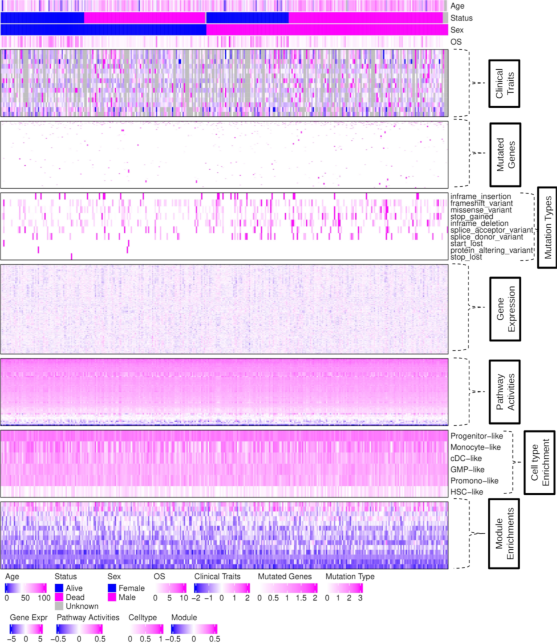
\includegraphics[width=0.97\textwidth]{jtrm_images/Fig1.pdf}
    \caption{Comprehensive Multi-omics characterization of patient samples along with clinical traits.}
    \label{fig:fig1}
\end{figure}
%%%%%%%%%%%%%%%%%%%%%%%%%%%%%%%%%%%
\subsection{Drug Data and Fingerprint Generation} 
We collected drug response data from the BeatAML dataset. A total of 165 unique drugs were available, out of which $150$ unique drugs were used in the training set and $153$ unique drugs were available for the test set. A total of $15$ drugs were novel and unique to the test set and not used in the training set (to test generalization capability of our models on unseen drugs). For each drug, Morgan fingerprints (MFP) \cite{yang2022concepts} were derived using RDKit \cite{bento2020open} package (v3.1) in Python (v3.10). We also utilized SMILES-based embedding representation for drugs as an alternative representation to MFP. The SMILES-based encoding of drugs were generated using a Teacher Forcing - Long Short Term Memory (TF-LSTM) deep learning model from \cite{mall2021modeling} as highlighted in Figure \ref{fig:fig2A}. The TF-LSTM model was trained on $\approx 2.5$ million compounds from PubChem \cite{kim2025pubchem} + MOSES dataset \cite{10.3389/fphar.2020.565644}. Overall, $96.7\%$ of the re-constructed compounds were valid as determined using RDKit and attained a mean categorical cross-entropy \cite{mall2021modeling} error of $0.001$ during reconstruction. In our machine learning models, we used either the MFP or the SMILES-embedding as a representation vector for drugs.

%%%%%%%%%%%%%%%%%%%%%%%%%%%%%%%%%%
\subsection{Drug Pathway Distance Estimation}
To estimate an approximate computational distance of drugs from individual oncogenic pathways, we utilize the drug target (gene) information available via DrugBank \cite{knox2024drugbank}. Here we use the genes and corresponding proteins as one or interchangeably. We then utilize the protein interaction network that is obtained through the \href{https://string-db.org/}{STRING} protein-protein interaction (PPI) database. From the STRING PPI network, we consider the network of human proteins and only those interactions which have strong experimental evidence (score $\ge700$).

Considering the drug targets as starting points in this interaction network, we perform network propagation using a random-walk with restart approach \cite{sherif2022immune,mall2013kernel} to obtain a propagation vector for each drug. The propagation vector can be used as a surrogate for the global distance of a protein from a given drug (and its targets). To obtain a local propagation vector, i.e., patient-specific propagation vector, we multiply the propagation score of each protein with their corresponding gene expression available via RNA-Seq for that patient. 

Our aim is to estimate the proximity of an oncogenic pathway from a given drug and a patient profile. If the genes which are part of an oncogenic pathway are all ranked higher in the sorted propagation vector, then the drug has close proximity to that oncogenic pathway, whereas if the genes are ranked randomly in the sorted propagation vector, then the drug has low proximity to the oncogenic pathway. This estimate was obtained using the AUCell package (v1.24.0) \cite{aibar2017scenic} in R. It estimates the area under the receiver operating curve (AUC), where higher AUC corresponds to closer proximity and lower AUC corresponds to further distance between a drug and the oncogenic pathway for a given patient. Figure \ref{fig:fig2B} highlights the steps involved in drug pathway distance estimation.
\begin{figure}[!ht]
    \centering
    \begin{subfigure}{0.99\linewidth}
        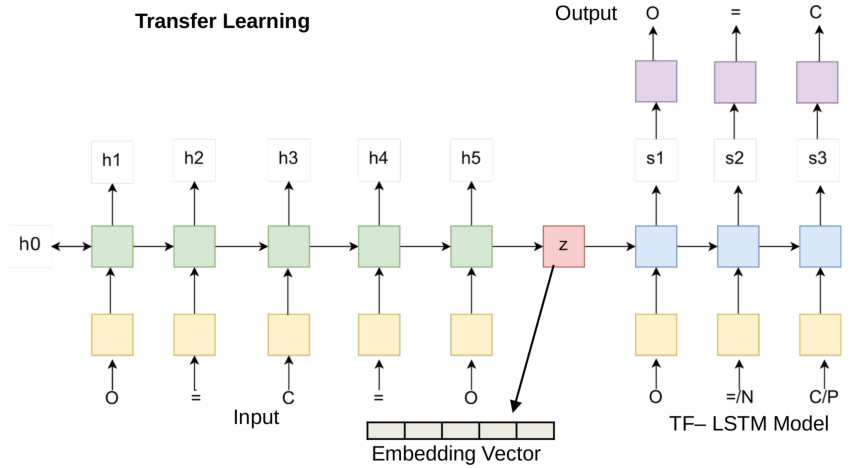
\includegraphics[width=0.9\textwidth]{jtrm_images/Figure2A.pdf}
        \caption{Representation of TF-LSTM \cite{mall2021modeling} model generating embedding vector for compounds. }
        \label{fig:fig2A}
    \end{subfigure}
    \begin{subfigure}{0.99\textwidth}
        \centering
        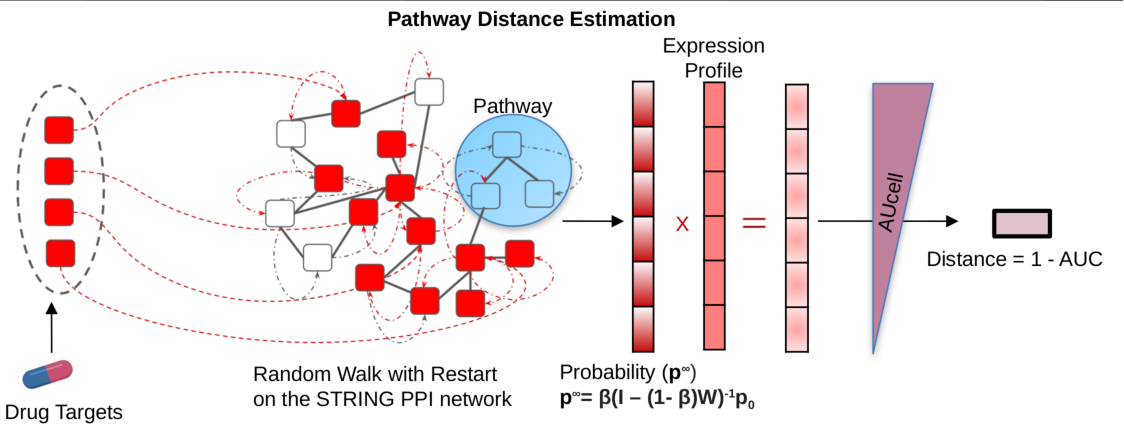
\includegraphics[width=0.99\textwidth]{jtrm_images/Figure2B.pdf}
        \caption{Steps involved in patient-specific drug-pathway distance estimation.}
        \label{fig:fig2B}
    \end{subfigure}
    \caption{Drug embedding generation technique and drug-pathway distance calculation.}
    \label{fig:fig2}
\end{figure}
%effect of drugs on specific pathways, we used a random walk with restart approach on STRING PPI networks. Pathway activity was estimated using gene expression profiles combined with diffusion scores from drug targets. The AUCell package was employed to measure the proximity of each pathway to the drugs in question. Drugs that had the highest impact on pathways were ranked, and their influence on disease outcomes was assessed.
%%%%%%%%%%%%%%%%%%%%%%%%%%%%%%%%%%%%
\subsection{Training and Test Data Preparation}
Using the aforementioned approach, we obtain the essential molecular features, i.e., mutation profile (mutation frequency and types), gene expression profile (most varying genes, oncogenes), and enrichment scores (pathway, module, cell state), along with clinical annotations to have a comprehensive representation for patient ($p$) profiles. We utilize the SMILES-embedding or MFP based encodings as drug id ($d$) representation along with information about direct drug-targets available via DrugBank \cite{knox2024drugbank}. Additionally, we have the drug response data, which encapsulates for a given patient id ($p$) and compound id ($c$), the corresponding area under the drug response curve. Utilizing these three information sources, we obtain the merged dataset by performing an inner join between drug response data and patient table using $p$ as the foreign key. This is followed by an inner join between the resulting dataset and the drug table using $d$ as the foreign key. We used the `merge' function in `pandas' package in Python to perform the table joins. 

The inner join operations are performed separately for the training and test sets. The resulting training set and test set have $34,387$ and $19,184$ patient-drug records respectively with 2,333 numeric features utilized for building and validating the drug response models. The training set is ready for ingestion in downstream machine learning models to predict patient-drug response, and the test set serves as an unseen dataset to evaluate and benchmark generalization performance of the designed models.
\begin{figure}[!ht]
    \centering
    
\includegraphics[width=0.95\textwidth]{jtrm_images/Figure3.pdf}the 
    \caption{The workflow followed to build the proposed PREDICT-AML model.}
    \label{fig:fig3}
\end{figure}
%%%%%%%%%%%%%%%%%%%%%%%%%%%%%%%%%%%%
\subsection{Machine Learning Models}
We developed and trained multiple machine learning models to predict drug response for patients using combined molecular, genomic, and clinical data, together with the drug and functional process representations. 
The designed models included generalized linear regression (GLR) \cite{nelder1972generalized}, support vector regression (SVR) \cite{chandorkar2015fixed}, Random Forests (RF) \cite{breiman2001random}, XGBoost \cite{chen2016xgboost}, LightGBM \cite{ke2017lightgbm}, CatBoost \cite{prokhorenkova2018catboost}, and feedforward neural networks \cite{hastie2009elements} among the standard machine learning models. We also trained several deep learning models using the SMILES representation of drugs as input to convolutional neural networks \cite{sermanet2012convolutional}, LSTM \cite{gers2000learning}, and graph attention networks \cite{velivckovic2017graph} combined with patient information and feedforward layers to build deep learning-based drug response models. 

All models were trained using 5-fold cross-validation on the training set (Waves 1 + 2) and tested on Waves 3 + 4. Performance metrics, including mean absolute error (MAE), root mean squared error (RMSE), Pearson correlation (r), Spearman correlation (sr) and coefficient of determination (R$^2$) were computed to assess model performance. Lower MAE and RMSE values are better, and higher r, sr and R$^2$ values are better.  All the tree-based models achieved near-optimal performance, with the CatBoost model achieving the lowest test MAE. Figure \ref{fig:fig3} represents all the steps involved in building the PREDICT-AML model.
%%%%%%%%%%%%%%%%%%%%%%%%%%%%%%%%%%%%%%%%%%%%%%%%%%%%%%%%%%%%%%
\subsection{Feature Association with Predicted Drug Responses}
To gain mechanistic insight into the features influencing drug response predictions, we investigated the association between predicted AUC values and various multiomic features across the top $10$ best-predicted drugs in both the training and test sets. These drugs include Venetoclax, Selumetinib (AZD6244), Trametinib (GSK1120212), Rapamycin, Motesanib (AMG-706), 17-AAG (Tanespimycin), Dasatinib (Sprycel), Cabozantinib (Cometriq), Elesclomol, and Sorafenib (Nexavar). These drugs were selected based on the high predictive performance (r, R$^2$) for the optimal CatBoost framework.

For each drug, we performed linear regression (using `lm' function in R v4.3.2) between predicted AUC values and continuous features such as gene expression, pathway activity scores, cell state enrichments, and module scores, while using Wilcoxon rank-sum tests for binary features like gene mutation status. We analyzed the associations separately for training (Wave 1+2) and test cohorts (Wave 3+4). The primary objective was to identify linearly associated features that were significantly correlating with predicted drug sensitivity from our optimal CatBoost model.
%@Siddhi: features part
%%%%%%%%%%%%%%%%%%%%%%%%%%%%%%%%%%%%%%%
\section{Results}
We performed a comprehensive comparison of various state-of-the-art machine learning as well as end-to-end deep learning models for the task of drug response prediction. Additionally, we performed association analysis w.r.t. engineered features and predicted drug response values for the drugs where our model performs optimally.
\subsection{Benchmarking Machine Learning Models}
We highlight the performance of different machine learning models in Figure \ref{fig:fig4}.
Figure \ref{fig:fig4}A highlights the distribution of the area under the drug response curve (AUC) between patient profiles in Waves 1+2 (Y\_train) and Waves 3+4 (Y\_test). We observe that the AUC values range between 0 and 300, where higher values indicate better response. Moreover, from Figure \ref{fig:fig4}A, we observe that the distribution of the drug responses are similar between the training and test sets (with no statistical difference i.e. p-value $> 0.05$ based on Wilcoxon-ranksum test \cite{mann1947test}).

\begin{figure}[!ht]
    \centering
    
\includegraphics[width=0.92\textwidth]{jtrm_images/Figure4.pdf}
    \caption{Performance comparison of machine learning models for predicting drug response of AML patients. We highlight the top 10 drugs for which our optimal model performs best and the top 10 patient profiles for which the prediction was most accurate. Here, `MFP' represents Morgan Fingerprints, `LS' corresponds to TF-LSTM embeddings, and `SMILES' is the SMILES representation for drugs. Additionally, `Feat' corresponds to the multiomic feature representation for patients.}
    \label{fig:fig4}
\end{figure}
We then showcase the performance of the different machine learning and deep learning models in Figures \ref{fig:fig4}B-K and Table \ref{table:t1}. Using different representations for drugs, namely the Morgan fingerprint (MFP) and TF-LSTM based embeddings (LS), we have two models for each standard machine learning technique like GLR, SVR, RF, XGBoost, CatBoost and LightGBM, respectively. The best model results for individual machine learning techniques are highlighted in Figures \ref{fig:fig4}B-K, while their counterparts' result is depicted in Supp Figures 2A-G. From Figures \ref{fig:fig4}B,C,H,  Supp. Figures 2A,B,G and Table \ref{table:t1}, we observe that the linear models and the feedforward neural network (FFNN) tend to be worst w.r.t. MAE and correlation metrics (r, sr, R$^2$) when compared to other methods. While linear models cannot capture the inherent non-linearity in the data, the FFNN achieves the best cross-validation MAE scores across all models (see Table \ref{table:t1}) but has poor generalization performance, indicating that the model has overfitted on the training data.

From Figure \ref{fig:fig4}D-G, we observe that the tree-based models achieve an MAE of $\approx$ 39 and a Pearson correlation of $\approx$ 0.66 for the test set. Similarly, from Supp. Figure C-F, we observe that the tree-based models achieve an MAE of $\approx$ 40 and a r score of $\approx$ 0.66 on the test set and are slightly worse than their individual counterparts. The embedding-based representation (LS) for drugs is slightly better than the MFP representation of drugs for RF, XGBoost, and LightGBM as observed in Table \ref{table:t1}. The RF model (LS + Feat) achieves a cross-validation r of 0.89 $\pm$ 0.01, R$^2$ of 0.79 $\pm$ 0.02, as depicted in Table \ref{table:t1}. Similarly, the LigthGBM model (LS + Feat) attains a cross-validation r of 0.89 $\pm$ 0.02, sr of 0.87 $\pm$ 0.02, and R$^2$ of 0.79 $\pm$ 0.03 as highlighted in Table \ref{table:t1}. However, the Catboost model using MFP representation for drugs has the best MAE of 39.04, RMSE of 52.03, r of 0.66 and R$^2$ of 0.44 for the test set as depicted in Table \ref{table:t1} and Figure \ref{fig:fig4}G. Interestingly, we observe that deep learning based methods tend to perform better than linear methods but worse than tree-based models (see Table \ref{table:t1}). The GAT, CNN, LSTM model in combination with FFNN achieve MAE of 40.7, 40.85, 40.7 and r of 0.63, 0.63, 0.62 respectively on the test set as illustrated in Figures \ref{fig:fig4}I-K and Table \ref{table:t1}. 

An added advantage with tree-based models is the ease of interpretability possible via availability of variable importance \cite{mall2018rgbm}. Variable importance in tree-based models measures the relative contribution of each input feature to the model's predictive performance. Different tree-based models use different criterion to estimate variable importance score including techniques like entropy, Gini impurity or mean squared error \cite{louppe2013understanding}. Supplementary Figure 3 highlights the top $20$ most important features for optimal CatBoost, RF and LGBM models as these models attained best performance on unseen test set as indicated in Table \ref{table:t1}. We observe from Supp. Figure 3A, that several Morgan Fingerprint features (MFP) for drug representation are imperative for model prediction. However, the distance of drugs from key pathways such as mTOR Signaling, Reactive Oxygen Species, Oxidative phosphorylation and Induced MAPK Signaling pathways are part of the top features for the CatBoost model (see Supp. Figure 3A). On the other hand, for the optimal RF and LGBM models, the primary set of most important variables are embedding representation of drugs (LS) and distance of drugs from oncogenic pathways in patients (AUC metrics) respectively (see Supp. Figures 3B-C). The RF and LGBM model lack diversity in most important variables whereas diverse set of features including drug, drug-pathway distance, expression of genes (\textit{CD300E}, \textit{HNRNPA2B1}) and molecular weight of drugs are imperative for drug predictions for the optimal CatBoost model as illustrated in Supp. Figure 3A.

Overall the tree-based models (Catboost in particular) can best capture the intricate relationship between drug representations, multiomic patient profile and functional processes to accurately estimate the drug response for a given patient as depicted by their cross-validation performance and the generalization performance on independent test set.
\begin{table}[!ht]
    \centering
    \resizebox{0.99\textwidth}{!}{
    \begin{tabular}{|c|c|c|c|c|c|c|c|c|c|c|c|}
    \hline
    \textbf{Methods} & \textbf{Features} & \textbf{CV (MAE)} & \textbf{Test (MAE)} & \textbf{CV (RMSE)} & \textbf{Test (RMSE)} & \textbf{CV (R$^2$)} & \textbf{Test (R$^2$)} & \textbf{CV (r)} & \textbf{Test (r)} & \textbf{CV (sr)} & \textbf{Test (sr)} \\
    \hline
    GLR & LS + Feat & 30.22 $\pm$ 1.97 & 44.86 & 40.34 $\pm$ 2.91 & 60 & 0.56 $\pm$ 0.05 & 0.28 & 0.74 $\pm$ 0.03 & 0.53 & 0.74 $\pm$ 0.03 & 0.56 \\
    GLR & MFP + Feat & 29.93 $\pm$ 1.92 & 43.48 & 40.10 $\pm$ 2.89 & 57.26 & 0.56 $\pm$ 0.05 & 0.34 & 0.75 $\pm$ 0.03 & 0.58 & 0.75 $\pm$ 0.03 & 0.58 \\
    SVR & LS + Feat & 30.13 $\pm$ 1.96 & 44.97 & 40.25 $\pm$ 2.90 & 60.37 & 0.56 $\pm$ 0.05 & 0.28 & 0.75 $\pm$ 0.03 & 0.53 & 0.74 $\pm$ 0.03 & 0.56 \\
    SVR & MFP + Feat & 29.93 $\pm$ 1.92 & 43.89 & 40.09 $\pm$ 2.89 & 57.73 & 0.56 $\pm$ 0.05 & 0.33 & 0.75 $\pm$ 0.03 & 0.57 & 0.75 $\pm$ 0.03 & 0.57 \\
    RF & LS + Feat & 21.82 $\pm$ 0.97 & 39.63 & 29.86 $\pm$ 1.51 & 52.09 & 0.79 $\pm$ 0.02 & 0.44 & 0.89 $\pm$ 0.01 & 0.66 & 0.89 $\pm$ 0.01 & 0.66 \\
    RF & MFP + Feat & 20.75 $\pm$ 1.22 & 40.16 & 28.29 $\pm$ 1.83 & 52.53 & 0.82 $\pm$ 0.02 & 0.44 & 0.90 $\pm$ 0.01 & 0.66 & 0.9 $\pm$ 0.01 & 0.65 \\
    XGBoost & LS + Feat & 24.29 $\pm$ 1.21 & 39.84 & 31.94 $\pm$ 1.76 & 52.34 & 0.73 $\pm$ 0.04 & 0.43 & 0.85 $\pm$ 0.02 & 0.66 & 0.84 $\pm$ 0.02 & 0.65 \\
    XGBoost & MFP + Feat & 22.94 $\pm$ 1.01 & 40.53 & 30.10 $\pm$ 1.45 & 52.88 & 0.78 $\pm$ 0.04 & 0.43 & 0.88 $\pm$ 0.2 & 0.66 & 0.87 $\pm$ 0.02 & 0.64 \\
    \textit{LightGBM} & \textit{LS + Feat} & 21.53 $\pm$ 1.12 & 39.5 & 28.75 $\pm$ 1.63 & \textit{52.09} & 0.79 $\pm$ 0.03 & \textit{0.44} & 0.89 $\pm$ 0.02 & \textit{0.66} & 0.87 $\pm$ 0.02 & \textit{0.66} \\
    LightGBM & MFP + Feat & 23.23 $\pm$ 1.08 & 40.07 & 31.12 $\pm$ 1.65 & 52.55 & 0.75 $\pm$ 0.04 & 0.43 & 0.86 $\pm$ 0.02 & 0.66 & 0.85 $\pm$ 0.02 & 0.64 \\
    Catboost & LS + Feat & 26.35 $\pm$ 1.56 & 39.24 & 37.26 $\pm$ 2.51 & 52.45 & 0.62 $\pm$ 0.04 & 0.44 & 0.79 $\pm$ 0.03 & 0.66 & 0.79 $\pm$ 0.02 & \textbf{0.66} \\
    \textbf{Catboost} & \textbf{MFP + Feat} & 21.02 $\pm$ 1.48 & \textbf{39.04} & 31.92 $\pm$ 2.43 & \textbf{52.03} & 0.73 $\pm$ 0.03 & \textbf{0.44} & 0.85 $\pm$ 0.02 & \textbf{0.66} & 0.85 $\pm$ 0.02 & 0.65 \\
    FFNN & LS + Feat & 23.51 $\pm$ 1.43 & 45.15 & 32.09 $\pm$ 2.1 & 58.69 & 0.72 $\pm$ 0.03 & 0.32 & 0.85 $\pm$ 0.02 & 0.57 & 0.84 $\pm$ 0.02 & 0.55 \\
    FFNN & MFP + Feat & 18.19 $\pm$ 1.05 & 42.65 & 25.42 $\pm$ 1.58 & 56.18 & 0.82 $\pm$ 0.02 & 0.36 & 0.91 $\pm$ 0.01 & 0.6 & 0.90 $\pm$ 0.01 & 0.59 \\
    GAT + FFNN & SMILES + Feat & 26.31 $\pm$ 0.37 & 40.7 & 37.13 $\pm$ 0.64 & 54.9 & 0.64 $\pm$ 0.01 & 0.39 & 0.80 $\pm$ 0.00 & 0.63 & 0.80 $\pm$ 0.01 & 0.62 \\
    CNN + FFNN & SMILES + Feat & 26.03 $\pm$ 0.23 & 40.85 & 37.03 $\pm$ 0.49 & 55.6 & 0.65 $\pm$ 0.01 & 0.4 & 0.80 $\pm$ 0.00 & 0.63 & 0.80 $\pm$ 0.00 & 0.63 \\
    LSTM + FFNN & SMILES + Feat & 26.27 $\pm$ 0.42 & 40.7 & 36.87 $\pm$ 0.61 & 55.14 & 0.65 $\pm$ 0.01 & 0.39 & 0.80 $\pm$ 0.00 & 0.62 & 0.799 $\pm$ 0.01 & 0.62 \\
    \hline 
    \end{tabular}
    }
    \caption{Performance comparison of ML models predicting drug response for AML patients. Here we highlight and italicized the models with the best and second best prediction metrics on the test set respectively.}
    \label{table:t1}
\end{table}
%%%%%%%%%%%%%%%%%%%%%%%%%%%%%%%%%%%%%%%%%%%%%%%
\subsection{Top Patient and Drug Predictions}
Figure \ref{fig:fig4}L highlights the top 10 best patient profiles for which the PREDICT-AML (hereby CatBoost) model has the best performance w.r.t. the Pearson correlation (r) and R$^2$ scores. These scores are estimated for each patient based on the total number of drugs tested (AUC scores in test set) and can vary per patient as indicated in `brackets' in Figure \ref{fig:fig4}L. We observe from Figure \ref{fig:fig4}L (top panel) that for each of these patients the r and R$^2$ values were $> 0.7$, indicating a strong alignment between the predicted and actual drug response. Similarly, we highlight the bottom 10 worst patient profiles in Figure \ref{fig:fig4}M (top panel). The correlation between the predicted and actual AUC scores for the worst patient (BA3117R) was still attaining a correlation (r) $\approx$ 0.2. It is noteworthy that for each patient there is more than 100 drug response curves available in the test set as depicted in Figures \ref{fig:fig4}L and M. This can enable the machine learning models to better capture patient specific multiomic information driving the drug response (sensitivity vs resistance).

Figure \ref{fig:fig4}L (bottom panel) shows the top 10 best drug predictions for which the PREDICT-AML model has the best performance w.r.t. r and R$^2$ scores. These scores are estimated for each drug based on the total number of patient samples tested (AUC scores in test set) and vary per drug as indicated in `brackets' in Figure \ref{fig:fig4}L. We observe from Figure \ref{fig:fig4}L (bottom panel) that for drugs such as Venetoclax, Selumetinib, and Trametinib, the CatBoost model can achieve correlation (r) values close to 0.7 and above, demonstrating accurate predictive performance. For each of the top 10 best drug predictions, there were over 100 patient samples available in the test set (see Figure \ref{fig:fig4}L). However, from Figure \ref{fig:fig4}M (bottom panel), we observe that there are certain drugs such as Perhexiline maleate, Baiclein, AF101, Ranolazaine, etc. the model predictions are fairly inaccurate resulting in poor correlation scores. This can partly be explained owing to lack of enough patient profiles for which these drugs have response curves as majority of these drugs have been tested for $< 100$ patient samples. 

Overall these results emphasize that while PREDICT-AML model is effective for certain patients and drugs, challenges persist while predicting response for others. 
%%%%%%%%%%%%%%%%%%%%%%%%%%%%%%%%%%%%%%%%%%%%%%%%%%%%%%%%%%%%%%%%%%%%%%%%%%%%
\subsection{Ablation Study on Multiomic Features for Patient Drug Response Prediction}
For the best CatBoost model, we performed comprehensive ablation studies taking different combinations of molecular features including varying gene expresison (VAR), oncogene expresison (Onco), mutation information (Mutations), pathway activities (Pathways), module enrichment (Modules), distance of pathway from drugs (AUC) together with Morgan Fingerprint (MFP) representation for drugs to predict drug sensitivity as depicted in Table \ref{table:t2} and Supp. Figures 2H-S.

\begin{table}[!ht]
\centering
 \resizebox{0.99\textwidth}{!}{
\begin{tabular}{|l|c|c|c|c|c|c|c|c|c|c|}
\hline
\textbf{Features Used} & \textbf{CV (MAE)} & \textbf{Test (MAE)} & \textbf{CV (RMSE)} & \textbf{Test (RMSE)} & \textbf{CV (R$^2$)} & \textbf{Test (R$^2$)} & \textbf{CV (r)} & \textbf{Test (r)} & \textbf{CV (sr)} & \textbf{Test (sr)} \\
\hline
MFP + AUC & 27.46 $\pm$ 1.21 & 40.47 & 38.85 $\pm$ 1.86 & 54.11 & 0.59 $\pm$ 0.05 & 0.41 & 0.77 $\pm$ 0.04 & 0.64 & 0.69 $\pm$ 0.03 & 0.63 \\
\textbf{MFP + Onco + Var + AUC} & 20.86 $\pm$ 1.39 & 39.54 & 31.73 $\pm$ 2.31 & 52.46 & \textbf{0.74 $\pm$ 0.04} & 0.43 & \textbf{0.85 $\pm$ 0.03} & 0.66 & \textbf{0.87 $\pm$ 0.02} & 0.65 \\
\textbf{MFP + Pathways + AUC} & \textbf{19.56 $\pm$ 1.01} & 40.15 & \textbf{30.41 $\pm$ 1.89} & 53.29 & 0.73 $\pm$ 0.04 & 0.41 & 0.85 $\pm$ 0.03 & 0.63 & 0.86 $\pm$ 0.02 & 0.63 \\
MFP + Modules + AUC & 20.99 $\pm$ 1.18 & 39.34 & 32.00 $\pm$ 2.00 & 52.51 & 0.70 $\pm$ 0.04 & 0.43 & 0.84 $\pm$ 0.03 & 0.66 & 0.85 $\pm$ 0.02 & 0.65 \\
MFP + Mutations + AUC & 22.00 $\pm$ 1.19 & 39.60 & 33.20 $\pm$ 1.94 & 52.85 & 0.70 $\pm$ 0.04 & 0.41 & 0.83 $\pm$ 0.03 & 0.65 & 0.84 $\pm$ 0.03 & 0.65 \\
MFP + AUC + Pathways + Modules & 25.35 $\pm$ 1.32 & 39.40 & 32.40 $\pm$ 2.14 & 52.48 & 0.64 $\pm$ 0.04 & 0.43 & 0.80 $\pm$ 0.03 & 0.66 & 0.81 $\pm$ 0.02 & 0.65 \\
MFP + AUC + Pathways + Mutations & 25.59 $\pm$ 1.38 & 39.51 & 36.40 $\pm$ 1.90 & 52.60 & 0.62 $\pm$ 0.05 & 0.41 & 0.79 $\pm$ 0.03 & 0.65 & 0.80 $\pm$ 0.02 & 0.65 \\
MFP + AUC + Pathways + Onco + Var & 24.77 $\pm$ 1.47 & 39.72 & 35.57 $\pm$ 2.35 & 52.74 & 0.64 $\pm$ 0.04 & 0.43 & 0.8 $\pm$ 0.03 & 0.65 & 0.80 $\pm$ 0.02 & 0.64 \\
\textbf{MFP + AUC + Modules + Mutations} & 25.86 $\pm$ 1.42 & \textbf{38.94} & 36.69 $\pm$ 2.17 & 52.23 & 0.64 $\pm$ 0.05 & \textbf{0.44} & 0.80 $\pm$ 0.03 & \textbf{0.66} & 0.80 $\pm$ 0.03 & \textbf{0.66} \\
MFP + AUC + Modules + Onco + Var & 24.77 $\pm$ 1.45 & 39.52 & 35.58 $\pm$ 2.24 & 52.65 & 0.64 $\pm$ 0.04 & 0.43 & 0.81 $\pm$ 0.03 & 0.66 & 0.81 $\pm$ 0.02 & 0.65 \\
MFP + AUC + Mutations + Onco +Var & 24.75 $\pm$ 1.48 & 39.29 & 35.58 $\pm$ 2.40 & 52.69 & 0.66 $\pm$ 0.04 & 0.44 & 0.81 $\pm$ 0.03 & 0.81 & 0.81 $\pm$ 0.02 & 0.65 \\
MFP + AUC + Mutations + Modules + Onco + Var & 24.74 $\pm$ 1.51 & 39.18 & 35.56 $\pm$ 2.45 & 52.32 & 0.64 $\pm$ 0.04 & 0.44 & 0.81 $\pm$ 0.03 & 0.66 & 0.81 $\pm$ 0.02 & 0.65 \\
MFP + AUC + Mutations + Pathways + Onco + Var & 25.67 $\pm$ 1.56 & 39.80 & 36.52 $\pm$ 2.46 & 53.27 & 0.64 $\pm$ 0.05 & 0.42 & 0.80 $\pm$ 0.03 & 0.65 & 0.80 $\pm$ 0.02 & 0.64 \\
MFP + AUC + Modules + Pathways + Onco + Var & 24.72 $\pm$ 1.46 & 39.42 & 35.53 $\pm$ 2.35 & 52.58 & 0.66 $\pm$ 0.05 & 0.43 & 0.81 $\pm$ 0.03 & 0.66 & 0.81 $\pm$ 0.023 & 0.65 \\
%MFP + AUC + Mutations + Modules + Pathways + Onco + Var & 27.653 $\pm$ 1.425 & 39.403 & 38.459 $\pm$ 2.177 & 52.601 & 0.599 $\pm$ 0.048 & 0.436 & 0.774 $\pm$ 0.03 & 0.66 & 0.775 $\pm$ 0.026 & 0.652 \\
\textbf{MFP + All Molecular Features} & 21.02 $\pm$ 1.48 & 39.04 & 31.92 $\pm$ 2.43 & \textbf{52.03} & 0.73 $\pm$ 0.03 & \textbf{0.44} & 0.85 $\pm$ 0.02 & \textbf{0.66} & 0.85 $\pm$ 0.02 & 0.65 \\
\hline
\end{tabular}
}
\caption{Ablation study of different feature sets using the CatBoost framework (overall optimal model).}
\label{table:t2}
\end{table}
From Table \ref{table:t2}, we observe that the CatBoost model built using MFP (for drugs) and pathway enrichments and drug-pathway distance (AUC) achieves the lowest cross-validation MAE ($19.56 \pm 1.01$) and RMSE ($30.41 \pm 1.89$). However, this model lacks generalization capability, as observed from its MAE of 40.15 and RMSE of 53.29 on the unseen test set (see Table \ref{table:t2} and Supp. Figure 2K). Similarly, the CatBoost model built using oncogene and variable gene expression, drug-pathway distance, and MFP for drugs attains the highest cross-validation R$^2$ ($0.74 \pm 0.04$), r ($0.85 \pm 0.03$) and sr ($0.87 \pm 0.02$). However, this model doesn't achieve the best generalization performance on the test set as depicted in Table \ref{table:t2} and Supp. Figure 2L. Interestingly, the CatBoost model built using MFP, drug-pathway distance, module enrichment, and mutation profiles of patients achieves the highest generalization performance of $\text{r}=0.66$, $\text{sr}=0.66$ and MAE of $38.94$ as showcased in Table \ref{table:t2} and Supp. Figure 2S. The performance of this model is similar to our optimal CatBoost model (MFP + All Features) for R$^2$ and Pearson correlation (r) on the unseen test set (see Table \ref{table:t2}). The ablation study highlights the benefits of adding multiomic representation for the molecular profile of the patient with an incremental gain in performance of the corresponding CatBoost model. 
%%%%%%%%%%%%%%%%%%%%%%%%%%%%%%%%%%%%%%%%%%%%%%%%%%%%%%%%%%%%%%%%%%%%%%%%%%%%%
\subsection{CatBoost Model Interpretation using Shapley Values}
An advantage of tree-based non-linear machine learning techniques, in contrast to black-box modeling techniques like support vector machines \cite{mall2015very} and artificial neural networks \cite{fausett2006fundamentals}, is that we can easily obtain feature/variable importance scores for all input features. The importance of a feature is the sum of information gained when splits (tree branching) are performed using that variable. A distinct benefit of using a CatBoost regressor is that out of all the 2,333 features used during training, variables which are not used for optimal tree splits in the optimal CatBoost model are pruned automatically and get a feature importance score of 0. 

Recently, several techniques such as the LIME \cite{ribeiro2016should} and SHAP \cite{lundberg2017unified} methods, have been proposed to overcome the aforementioned limitations. These methods have the ability to interpret feature importance scores from complex training models as well as provide interpretable predictions for a test sample by grounding their reasoning on the top $k$ features for that particular test instance. In our work, we use the SHAP (SHapley Additive exPlanations) method, a unified framework for interpreting predictions, as it was shown in \cite{lundberg2017unified} to outperform LIME and they demonstrated that its predictions are better aligned with human intuitions.

The SHAP method belongs to the class of additive feature attribution methods where a test instance prediction is composed as a linear function of features and satisfies three critical properties comprised of local accuracy, missingness, and consistency. The explicit SHAP regression values come from a game-theory framework \cite{lipovetsky2001analysis,shapley1953stochastic} and can be computed as:
\begin{equation}
    \phi_{i} = \sum_{S \subseteq Q/\{i\}}\frac{|S|!(|Q|-|S|-1)!}{|Q|!} [H_{S\cup{\{i\}}}(x_{S \cup \{i\}}) - H_{S}(x_{S})]
\end{equation}

Here, Q represents the set of all d features, and S represents the subsets obtained from Q after removing the feature $i^{\text{th}}$and $\phi$ is an estimate of the importance of feature i in the model. 
In order to refrain from undergoing differences to estimate $\phi$, the SHAP method $\approx$ the Shapley value by either performing Shapley sampling \cite{strumbelj2010efficient} or quantitative input influence \cite{datta2016algorithmic}. A detailed description of the SHAP method for model interpretation is available in \cite{lundberg2017unified}.

We passed our optimal CatBoost-based PREDICT-AML model along with the training set to the SHAP method as shown in Figure \ref{fig:shapA} to obtain the importance of features based on Shapley values. Figure \ref{fig:shapA} highlights the top 20 features based on Shapley values. Moreover, it also provides directionality, i.e., when a feature attains ‘high’ or ‘low’ values, the corresponding Shapley values are positive or negative. The positive Shapley values drive the predictions towards sensitivity, whereas the negative Shapley values influence the predictions to move towards resistance. From Figure \ref{fig:shapA}, we can observe that when top features such as the majority of Morgan Fingerprints (MFP) take high values, the corresponding Shapley values are negative, driving model prediction to resistance, whereas when these features take low values (i.e., 0), the corresponding Shapley values are positive. Similarly, Figure \ref{fig:shapA} illustrates that when top characteristics such as the distance of the UVA-induced MAPK signaling pathway is lower to drugs (i.e., higher AUC), the corresponding Shapley values are positive and drive model prediction towards sensitivity. Additionally, higher expression of \textit{CD300E}, an activator of myeloid cells, and \textit{HNRNPA2B1} corresponds to lower Shapley values, driving model predictions towards resistance.

Figure \ref{fig:shapB} gives an illustrative example of a patient treated with Vismodegib where the activation of Morgan Fingerprint features 667, 680 and 837 (out of 1024 features), along with a lower distance of the UVA-induced MAPK signaling pathway (higher AUC $> 0.5$) from the drug and high expression of \textit{HNRNPA2B1} gene drive accurate drug sensitivity prediction (predicted value of 286.11 vs actual value of 286.33). Similarly, from Figure \ref{fig:shapC}, we observe that the activation of Morgan Fingerprint features 296 and 737 together with the greater distance of the UVA-induced MAPK signaling and the oxidative phosphorylation pathway of the drug Elesclomol drove the prediction of drug resistance for a given patient (predicted value of 21.28 vs. actual value of 9.39). 
\begin{figure}[!ht]
    \centering
    \begin{subfigure}{0.7\textwidth}
        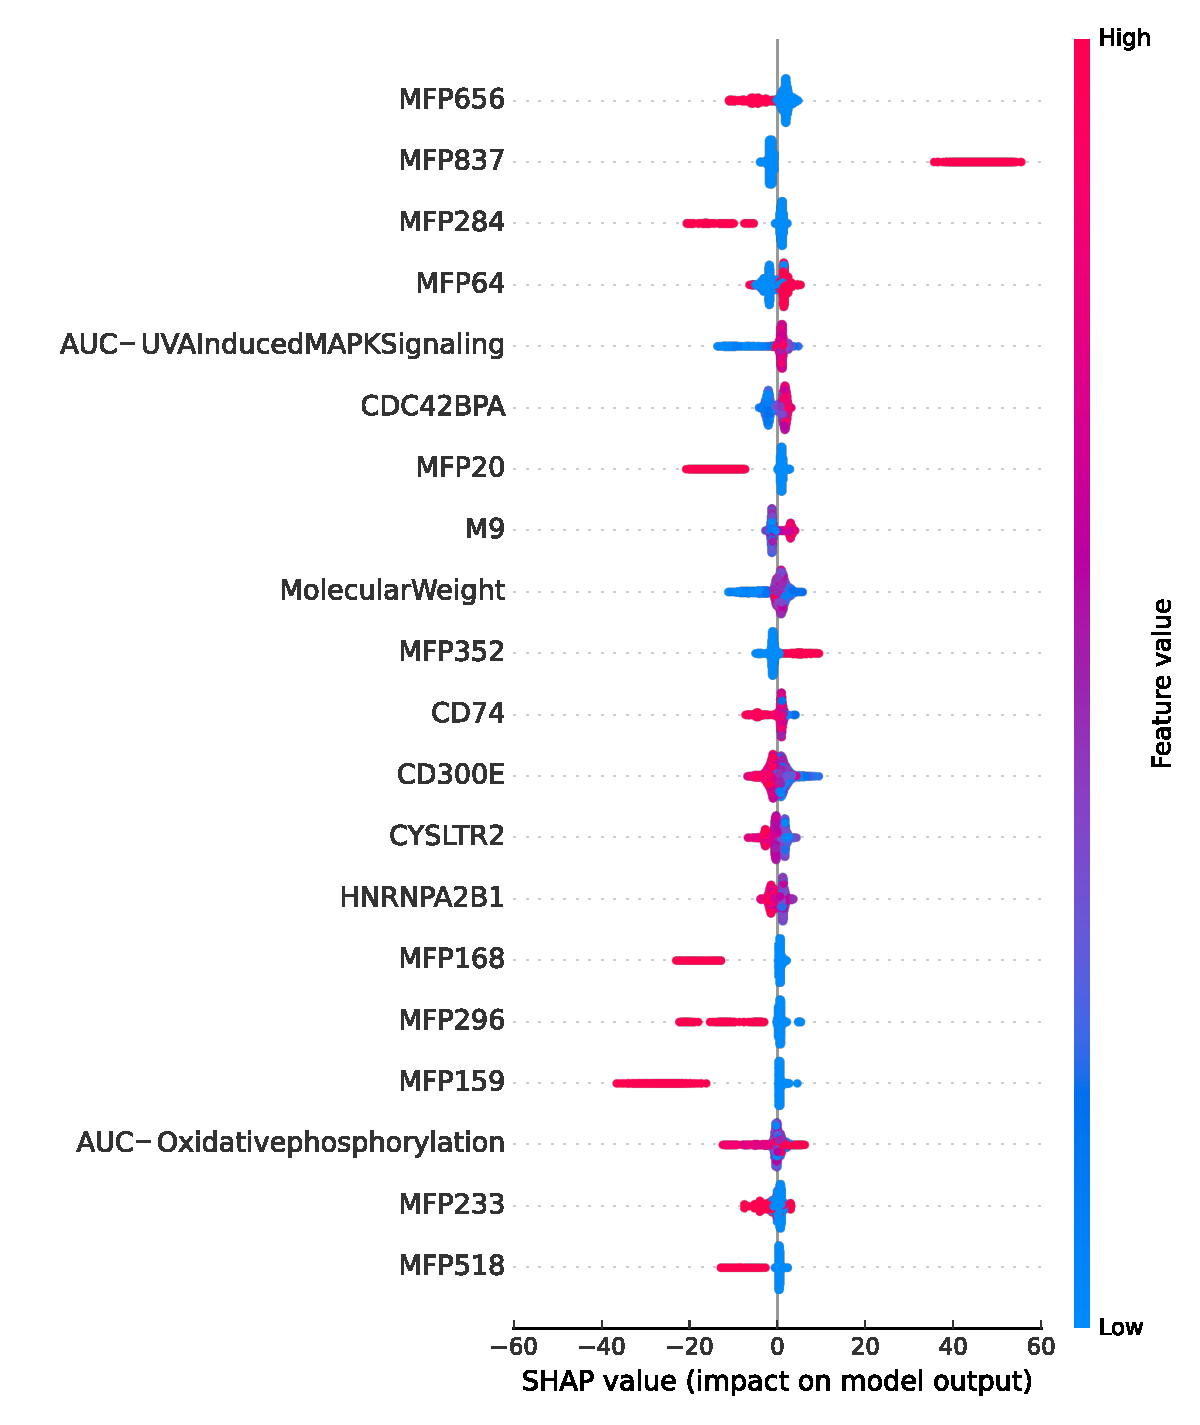
\includegraphics[width=0.99\textwidth]{jtrm_images/CatBoost_SHAP_Summary.pdf}
        \caption{Shapley values of top 20 features for optimal CatBoost model}
        \label{fig:shapA}
    \end{subfigure}
    %\begin{subfigure}{0.95\textwidth}
    %    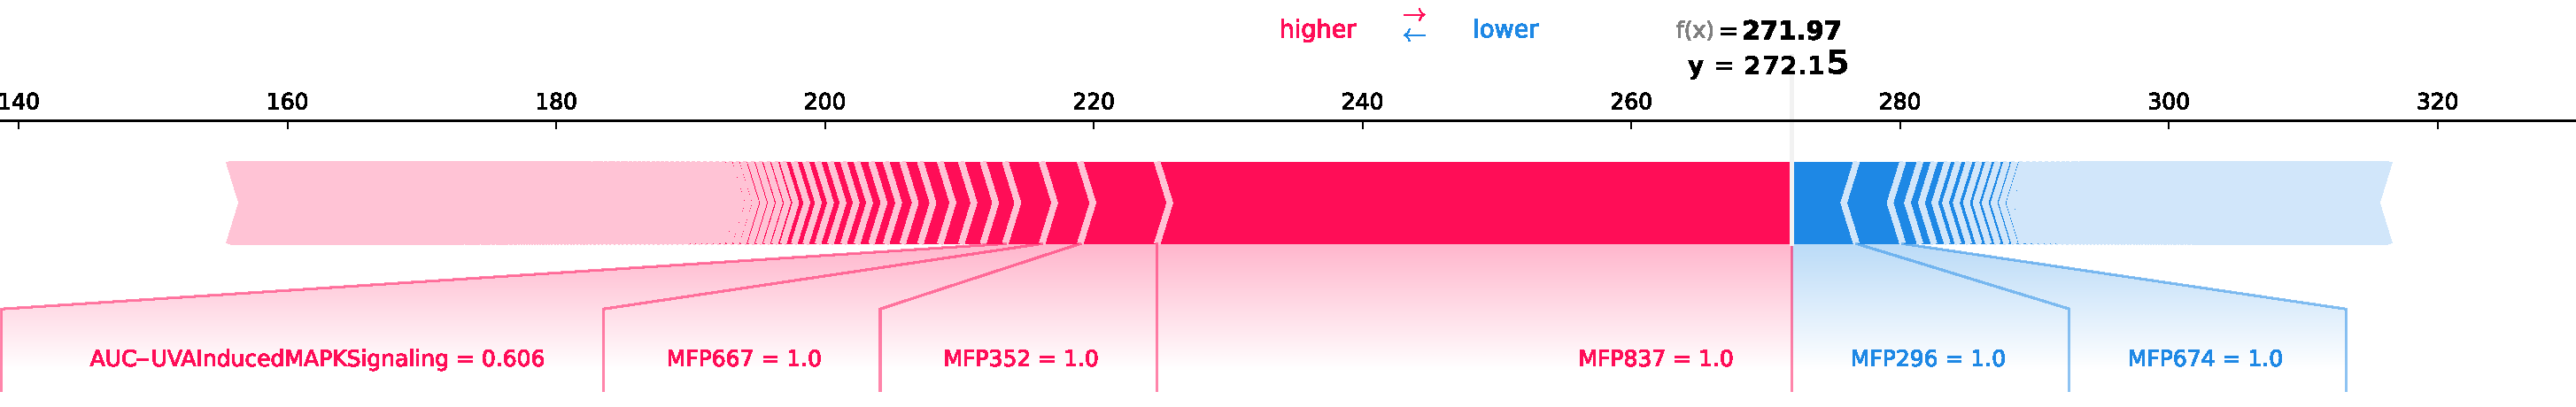
\includegraphics[width=0.9\textwidth]{jtrm_images/CatBoost_SHAP_sensitive_sample1.pdf}
    %    \caption{Illustrative Example 1 of features driving accurate prediction of drug sensitivity}
    %    \label{fig:shapB}
    %\end{subfigure}
    \begin{subfigure}{0.95\textwidth}
        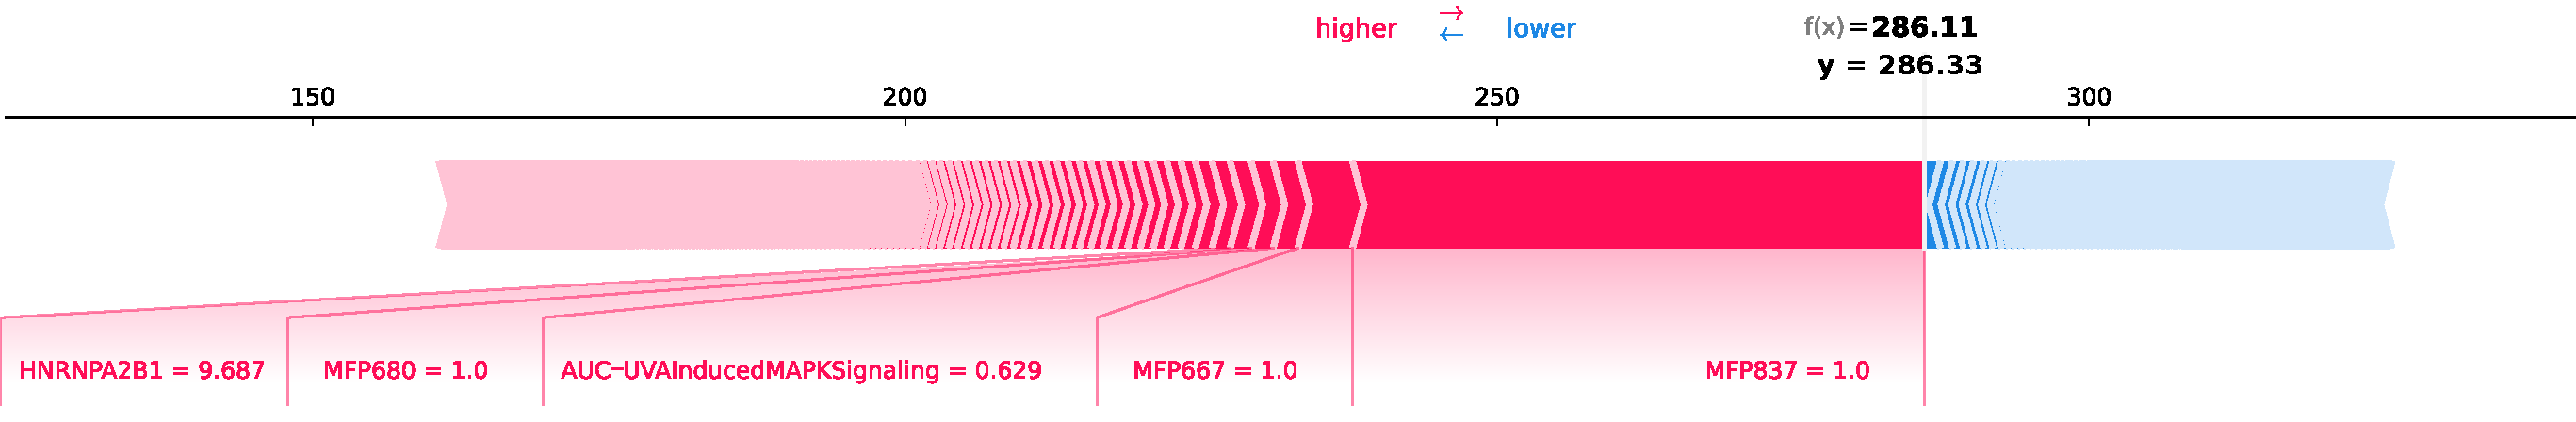
\includegraphics[width=0.99\textwidth]{jtrm_images/CatBoost_SHAP_sensitive_sample2.pdf}
        \caption{Illustrative Example of features driving accurate prediction of drug sensitivity}
        \label{fig:shapB}
    \end{subfigure}
    %\begin{subfigure}{0.95\textwidth}
    %    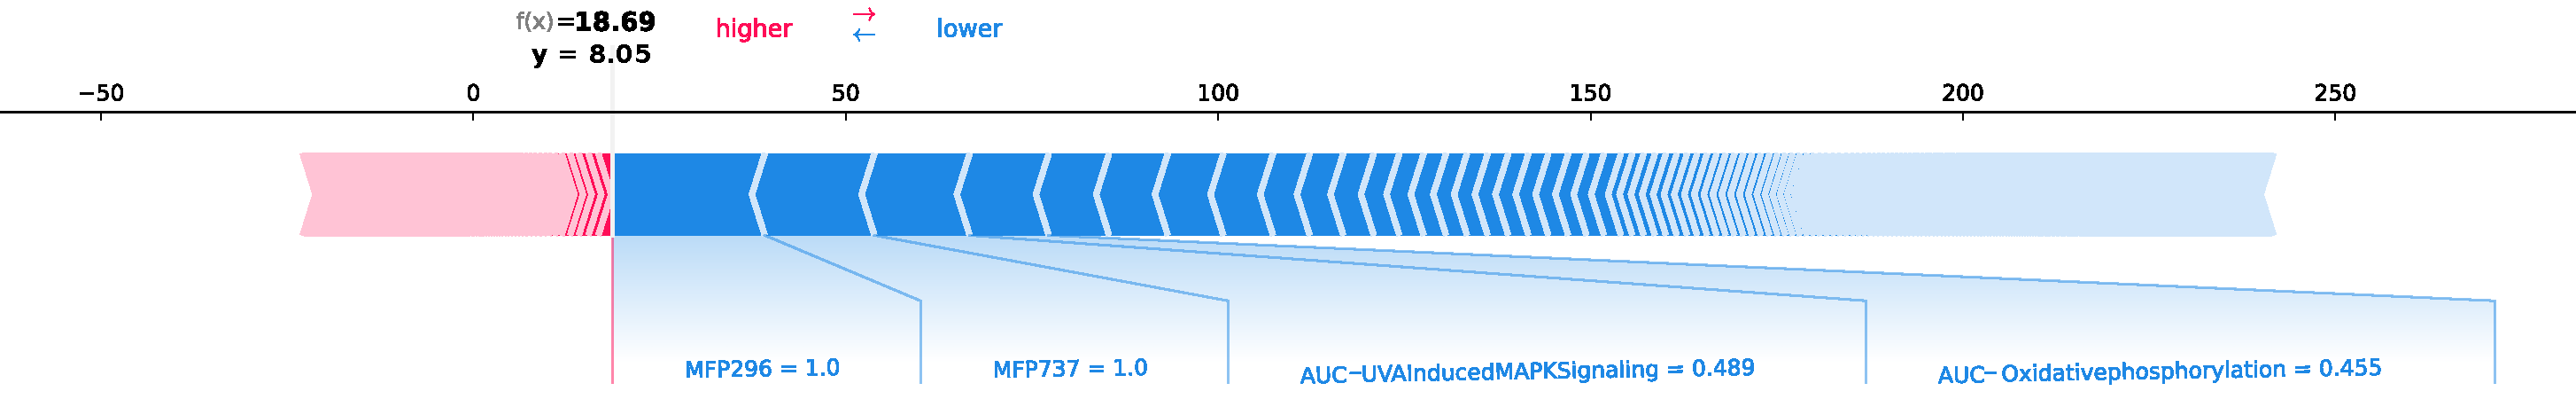
\includegraphics[width=0.9\textwidth]{jtrm_images/CatBoost_SHAP_resistance_sample1.pdf}
    %    \caption{Illustrative Example 1 of features driving accurate prediction of drug resistance}
    %    \label{fig:shapD}
    %\end{subfigure}
    \begin{subfigure}{0.95\textwidth}
        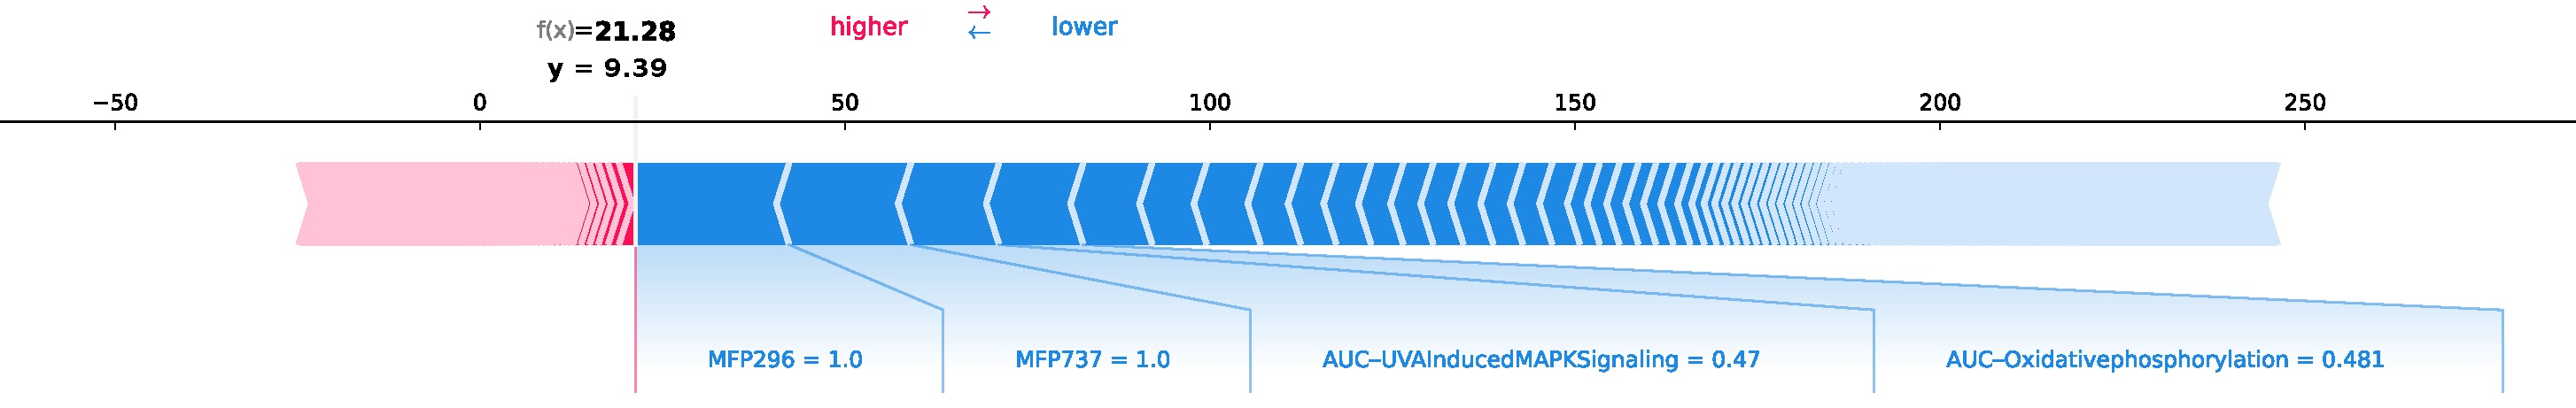
\includegraphics[width=0.99\textwidth]{jtrm_images/CatBoost_SHAP_resistance_sample2.pdf}
        \caption{Illustrative Example of features driving accurate prediction of drug resistance}
        \label{fig:shapC}
    \end{subfigure}
    \caption{Model interpretation made easy via Shap method \cite{lundberg2017unified}.}
    \label{fig:snap}
\end{figure}

%%%%%%%%%%%%%%%%%%%%%%%%%%%%%%%%%%%%%%%%%%%%%%%%%%%%%%%%%%%%%%%%%%%%%%%%%%%%%
\subsection{Feature Association Analysis for Model-Predicted Drug Responses }
We observed that seven biological features demonstrated statistically significant associations ($q < 0.05$) with model-predicted drug responses across the top 10 drugs in both training and test datasets. Importantly, these associations were not only consistent but often stronger in the test cohort, with R$^2$ values in the test set frequently exceeding those in training, reflecting the generalizability of the model. 
To assess the strength and direction of these relationships, we generated regression plots for each drug-feature pair, which revealed both shared and drug-specific trends. Features such as Immunogenic Cell Death (ICD) pathway activity and cDC-like (conventional dendritic cell–like) enrichment stood out as key modulators of drug sensitivity in AML. 
Among these, the ICD pathway score exhibited the strongest predictive association with Venetoclax response, yielding an R$^2$ of $0.58$ ($p=2.95e-38$) in the training set and $0.637$ ($p=2.94e-39$) in the test set. 
This aligns well with Venetoclax’s mechanism as a BCL-2 inhibitor that promotes mitochondrial apoptosis while concurrently inducing immunogenic cell death through the release of ATP and \textit{HMGB1} \cite{cao2023mechanisms}. 
Such a response not only leads to malignant cell elimination but also potentiates antitumor immunity through damage-associated molecular patterns (DAMP) signaling, providing a mechanistic rationale for its robust clinical efficacy in AML, as supported by a recent study \cite{chen2024comprehensive}.
\begin{figure}[!ht]
    \centering
    \begin{subfigure}{0.99\linewidth}
        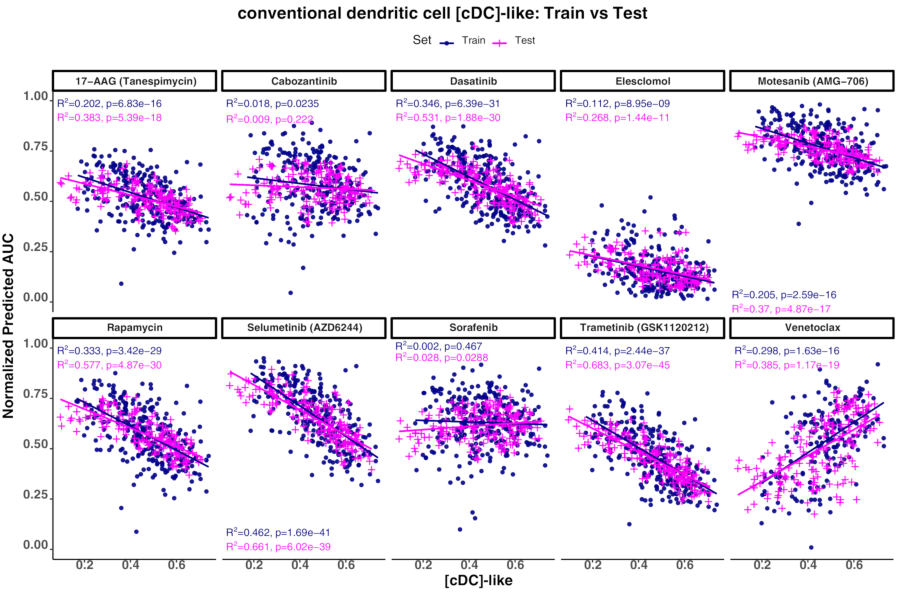
\includegraphics[width=0.9\textwidth]{jtrm_images/fig_5a_compressed_gimp.pdf}
        \caption{Regression analysis of cDC-like signature with top 10 drugs area under drug-response curve across training and test sets.}
        \label{fig:fig5A}
    \end{subfigure}
    \begin{subfigure}{0.99\textwidth}
        \centering
        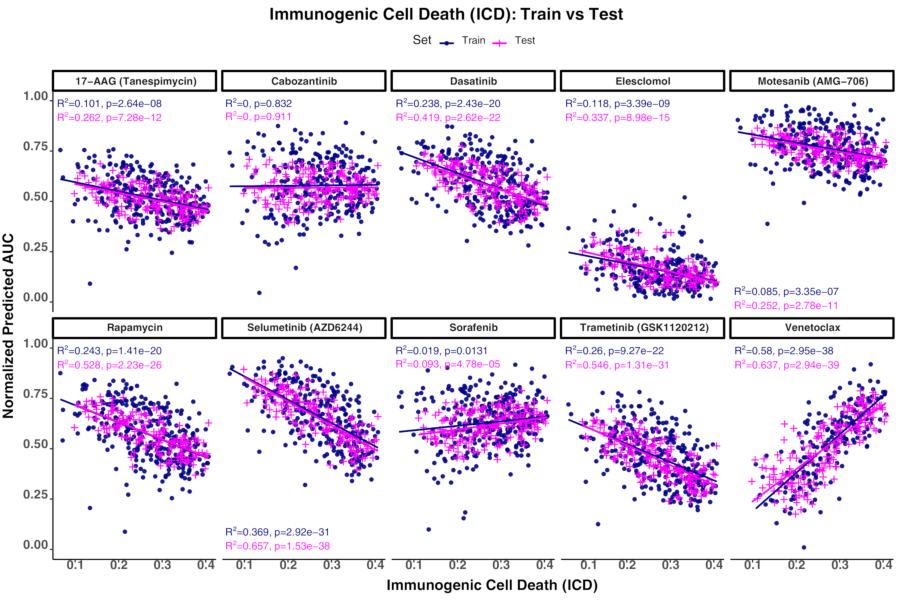
\includegraphics[width=0.9\textwidth]{jtrm_images/fig_5b_compressed_gimp.pdf}
        \caption{Regression analysis of Immunogenic Cell Death (ICD) pathway score with top 10 drugs area under drug-response curve across training and test sets.}
        \label{fig:fig5B}
    \end{subfigure}
    \caption{Linear regression analysis of multiomic features with top 10 drugs' AUC.}
    \label{fig:fig5}
\end{figure}

Similarly, we found that cDC-like signature scores were negatively correlated with predicted drug sensitivity across most drugs, achieving the strongest effects with MEK inhibitors. 
MEK inhibitors achieved the highest correlations with Selumetinib (Test: R$^2=0.661$, $p=6.02e-39$) and Trametinib (Test: R$^2=0.683$, $p=3.07e-45$). 
We found that Venetoclax maintains its distinctive positive correlation pattern with this immune signature (Test: R$^2=0.385$, $p=1.17e-19$), while Sorafenib represents an exception with a non-significant association (Test: R$^2=0.028$, $p=0.029$). 

Beyond immune pathways, we observed strong associations between drug responses and expression levels of \textit{CD300E}, \textit{LGALS2}, and \textit{VCAN} gene expression. As shown in Supp. Figure 4A, we found that \textit{CD300E} gene expression showed strong and reproducible negative correlations with drugs such as Selumetinib (Test: R$^2 = 0.626$, $p = 1.34e-35$), Trametinib (Test: R$^2 = 0.609$, $p = 2.84e-37$), Dasatinib (Test: R$^2 = 0.548$, $p = 8.42e-32$), and Rapamycin (Test: R$^2 = 0.633$, $p = 9.99e-35$), indicating that lower \textit{CD300E} expression may predict higher sensitivity to these agents. In contrast, we observed a positive correlation with Venetoclax (Test: R$^ = 0.589$, $p = 1.12e-34$), suggesting an opposite regulatory pattern. Similarly, we saw that \textit{ARHGEF10L} gene expression exhibited strong negative associations with Selumetinib (Test: R$^2 = 0.691$, $p = 3.77e-42$), Trametinib (Test: R$^2 = 0.659$, $p = 1.67e-42$), Rapamycin (Test: R$^2 = 0.566$, $p = 3.76e-29$), and Dasatinib (Test: R$^2 = 0.438$, $p = 1.47e-23$), while again showing a positive correlation with Venetoclax (Test: R$^2 = 0.431$, $p = 1.4e-22$) (see Supp. Figure 4B). We identified \textit{LGALS2} as the most predictive single characteristic, as shown Supp. Figure 4C, with significant negative correlations for Trametinib (test: R$^2 = 0.667$, $p = 2.3e-43$), Selumetinib (Test: R$^2 = 0.642$, $p = 4.44e-37$), and Rapamycin (Test: R$^2 = 0.612$, $p = 7.33e-33$). We also noted that Venetoclax again deviated from this trend (Test: R$^2 = 0.343$, $p = 3.41e-17$). We found that the M1 macrophage signature showed consistent negative correlations across most drugs, with the strongest associations observed for Selumetinib (Test: R$^2 = 0.802$, $p = 1.65e-57$), Trametinib (Test: R$^2 = 0.675$, $p = 2.33e-44$), and Rapamycin (Test: R$^2 = 0.58$, $p = 2.99e-30$), while Venetoclax again showed a positive association (Test: R$^2 = 0.568$, $p = 7.97e-33$) (see Supp. Figure 4D). Lastly, we observed from Supp. Figure 4E that \textit{VCAN} expression displayed strong negative correlations with Selumetinib (Test: R$^2 = 0.696$, $p = 9.66e-43$), Trametinib (Test: R$^2 = 0.609$, $p = 2.32e-37$), Rapamycin (Test: R$^2 = 0.554$, $p = 3.01e-28$), and Dasatinib (Test: R$^2 = 0.491$, $p = 2.85e-27$), and a positive association with Venetoclax (Test: R$^2 = 0.587$, $p = 1.97e-34$). Across all features, we consistently observed that Sorafenib lacked significant associations. These findings highlight that Venetoclax uniquely exhibits directionally opposite associations compared to other drugs, likely due to its distinct apoptotic mechanism via BCL-2 inhibition.
%%%%%%%%%%%%%%%%%%%%%%%%%%%%%%%%%%%%%%%%
\section{Discussion}\label{sec4}
In this study, we present PREDICT-AML, a machine learning framework developed to accurately forecast patient-specific drug responses in AML using the richly annotated, multi-omics BeatAML dataset. 
Our work addresses a critical limitation in earlier BeatAML studies by shifting from retrospective, correlative analyses to a predictive modeling approach capable of generalizing across unseen patients, an essential requirement for clinical translation. 
The PREDICT-AML framework integrates diverse data modalities, including gene expression, somatic mutation status, pathway activity, immune cell-state enrichment scores, and key clinical features. 
To capture the pharmacological context of each drug, we incorporated molecular embeddings derived from chemical structure and pathway proximity metrics reflecting mechanistic alignment between drug targets and biological processes. 
A range of algorithms, including generalized linear regression (GLR), random forests, neural networks, and boosting models, were benchmarked, with CatBoost, a gradient boosting method optimized for high-dimensional and heterogeneous data, emerging as the best-performing model. 
The final model achieved a mean absolute error (MAE) of 39.04 and a Pearson correlation of 0.66 on an unseen test set, confirming its generalization and robust predictive capacity.

We further validated data quality using dimensionality reduction techniques such as t-SNE and PCA, which revealed no batch effects between training and testing cohorts, suggesting successful harmonization across collection waves. 
Clustering based on the top 150 most variable genes revealed three major transcriptional subgroups, consistent across both partitions, indicating stable underlying molecular heterogeneity. 
In addition to high predictive performance, one of the core strengths of PREDICT-AML lies in its interpretability. By integrating the Shapley method \cite{shapley1953stochastic} and utilizing SHAP values, we decompose the model’s predictions into contributions from each input feature. 
This enables us to:
\begin{itemize}
    \item Quantify the impact of individual features (e.g., specific gene mutations, pathway activities, drug fingerprints) on the predicted drug response for each patient.
    \item Rank features by their importance, facilitating the identification of biomarkers or pathways that are consistently associated with sensitivity or resistance to particular drugs.
    \item Provide patient-specific explanations, which are crucial for precision medicine, as they help clinicians understand why a certain therapy can be recommended for a given patient profile.
\end{itemize}
Overall, the use of SHAP and Shapley values bridges the gap between predictive modeling and clinical interpretability. It enables the identification of key molecular determinants of drug response in AML, supports personalized treatments, and enhances the transparency and trustworthiness of the PREDICT-AML framework.

Through systematic feature association analysis, we identified several biologically meaningful features, such as \textit{CD300E}, \textit{LGALS2}, \textit{VCAN}, and \textit{ARHGEF10L} gene expression, along with M1 macrophage signature, ICD pathway activity, and cDC-like immune states, that were significantly associated with predicted drug responses across multiple drugs. 
These associations were often reproducible between the train and test cohorts, indicating that these features may serve as shared modulators of sensitivity across a range of therapeutic agents. 
For instance, ICD pathway activity was most strongly correlated with Venetoclax response, while cDC-like enrichment showed a robust inverse correlation with MEK inhibitors but a positive one with Venetoclax.

It is crucial to emphasize that our use of CatBoost, a non-linear model, allowed us to capture complex, multi-feature interactions and conditional dependencies that are not represented in univariate or even multivariate linear regression. 
This explains why certain features, although not statistically significant in isolation, still ranked highly in model-derived importance scores and had a substantial impact on predictions. 
In other words, PREDICT-AML not only captures additive effects but also models intricate interactions among and between molecular and clinical features, offering deeper insights into AML drug responsiveness. The convergence of predictive accuracy, biological interpretability, and cross-cohort consistency underscores the potential of PREDICT-AML as a decision-support system, capable of informing precision treatment strategies in AML based on patient-specific multi-omics signatures.

To contextualize our findings and underscore the novelty of PREDICT-AML, we compare our results with recent studies that have similarly focused on predicting drug response in AML using multi-omics and machine learning. A recent reanalysis of the BeatAML dataset by \cite{karathanasis2024machine} employed ElasticNet models with automated gene filtering to predict drug response for $122$ drugs (mean r of $0.36$). While the study demonstrated the potential of RNA-seq data as a more informative modality than exome sequencing or clinical data, their modeling approach remained largely linear and lacked the generalizability observed in our non-linear CatBoost model, which achieved a test set $r$ of 0.66 across all drugs using more complex feature integration.

Similarly, MDREAM, an ensemble-based multi-omics \cite{trac2023prediction}, on the BeatAML validation set using only $122$ drugs (i.e., only including drugs with over 100 patient drug sensitivity information in the validation set \cite{trac2023prediction}). While emphasizing the predictive value of integrated RNA and mutation data, the model inflates test performance by removing drugs with reduced patient drug response information. Additionally, unlike PREDICT-AML, MDREAM did not incorporate pathway proximity features or perform interpretability analyses such as SHAP to highlight driver features, limiting its interpretability and clinical utility.

Another compelling precision medicine effort is Quadratic Phenotypic Optimization Platform (QPOP), which predicts therapeutic sensitivities based on ex vivo drug combinations with rapid turnaround \cite{sahib2024combinatorial}. While \cite{sahib2024combinatorial} demonstrated high clinical accuracy (86.2\%), its reliance on ex vivo experimental profiling contrasts with our \textit{in silico} approach that scales more efficiently and captures complex non-linear dependencies using multi-modal data. 
Lastly, MSDRP \cite{zhao2023msdrp}, a deep learning framework integrating drug structures and cell line features through similarity fusion, showed strong performance in cancer cell lines but lacked direct validation in patient-derived datasets. It also highlighted challenges in clinical translation due to interpretability and sparse drug-target annotations. Notably, our model not only matches the predictive performance of top models but also offers explainability and validation across independent test set (Waves 3 + 4), marking a critical step toward clinical implementation.

For future directions, PREDICT-AML can be further enhanced by accurately integrating single-cell transcriptomic data to capture intra-patient heterogeneity and improve resolution in drug response prediction. Incorporating longitudinal samples could allow tracking of evolving drug sensitivities during treatment. Expanding the model to simultaneously predict drug efficacy and potential side effects would provide a more holistic view, enabling clinicians to balance therapeutic benefit with tolerability when making treatment decisions. From a modeling standpoint, leveraging causal inference and multi-task learning could improve performance and biological interpretability across drug classes. Lastly, integrating the model into a clinical decision-support system, paired with explainability tools, would bring PREDICT-AML closer to real-world application, empowering oncologists with personalized, data-driven insights for AML treatment.


%%%%%%%%%%%%%%%%%%%%%%%%%%%%%%%%%%%%%%%%
\section{Conclusion}\label{sec5}
In this study, we developed PREDICT-AML, a machine learning framework for predicting personalized drug responses in acute myeloid leukemia patients. By leveraging the rich multi-omics and clinical data from the BeatAML cohort, we engineered comprehensive representations of drugs, patient profiles, and biological pathways to accurately estimate drug sensitivity.
Our optimal PREDICT-AML model, based on the CatBoost algorithm, demonstrated strong predictive performance, achieving a mean absolute error of 39.04 and a Pearson correlation of 0.66 on the independent test set. This highlights the model's ability to generalize to unseen patient data.

While our results are promising, further validation on prospective clinical cohorts is necessary to fully assess the model's real-world applicability. Additionally, more comprehensive interpretability analyses using methods like Group Shapley \cite{jullum2021groupshapley} could provide valuable insights grouping sets of features driving drug response predictions. In conclusion, PREDICT-AML represents a significant step towards precision medicine in AML treatment. By accurately predicting patient-specific drug responses, this framework has the potential to guide clinicians in selecting optimal therapies, ultimately improving outcomes for AML patients.

\section*{Declarations}
\bmhead{Ethics approval and consent to participate}
N/A

\bmhead{Consent for Publication}
All authors have read the manuscript and provide consent for publication.

\bmhead{Availability of Data and Material}
All the code used to generate the workflow, along with a detailed step-by-step process to obtain the results and corresponding analysis, is provided at: \url{https://github.com/raghvendra5688/PT-AML}.

\bmhead{Competing interests}
The authors declare no competing interests

\bmhead{Supplementary information}
Supplementary information relevant to the manuscript is aggregated and provided as an additional file.

\bmhead{Funding}
The authors thank the Qatar National Library (QNL) for their support in providing resources and funding the APC, which was instrumental in completing this research. All authors have consented to this acknowledgment.

\bmhead{Acknowledgements}
Open Access funding provided by the Qatar National Library.

\bmhead{Authors' Contributions}
R.M. and H.B. conceived the study. S.P.J. and R.M. collected, curated and assimilated the data. S.P.J. and R.M. performed the feature engineering. R.M. built the machine learning models. S.P.J. performed association analysis. S.P.J., H.B. and R.M. wrote and revised the manuscript. H.B. and R.M. supervised the study.
% 

% Some journals require declarations to be submitted in a standardised format. Please check the Instructions for Authors of the journal to which you are submitting to see if you need to complete this section. If yes, your manuscript must contain the following sections under the heading `Declarations':

% \begin{itemize}
% \item Funding
% \item Conflict of interest/Competing interests (check journal-specific guidelines for which heading to use)
% \item Ethics approval and consent to participate
% \item Consent for publication
% \item Data availability 
% \item Materials availability
% \item Code availability 
% \item Author contribution
% \end{itemize}

%%===========================================================================================%%
%% If you are submitting to one of the Nature Portfolio journals, using the eJP submission   %%
%% system, please include the references within the manuscript file itself. You may do this  %%
%% by copying the reference list from your .bbl file, paste it into the main manuscript .tex %%
%% file, and delete the associated \verb+\bibliography+ commands.                            %%
%%===========================================================================================%%

\bibliography{sn-bibliography}% common bib file
%% if required, the content of .bbl file can be included here once bbl is generated
%%\input sn-article.bbl

\end{document}
